\documentclass[conference]{IEEEtran}
\usepackage{cite,amsmath,amssymb,graphicx,tikz,xcolor}
\usetikzlibrary{arrows.meta,positioning,shapes.geometric}
\def\BibTeX{{\rm B\kern-.05em{\sc i\kern-.025em b}\kern-.08em T\kern-.1667em\lower.7ex\hbox{E}\kern-.125emX}}
\title{NutriSense: Uncertainty-Aware Meal Portion and Nutrient Assessment for School Meal Monitoring}
\author{%
\IEEEauthorblockN{SS Gokula Swamy}\IEEEauthorblockA{\textit{BMS College of Engineering}\\Bengaluru, India\\gokulaswamyss@gmail.com}
\and\IEEEauthorblockN{Roshanth V}\IEEEauthorblockA{\textit{BMS College of Engineering}\\Bengaluru, India\\roshanth@example.com}
\and\IEEEauthorblockN{Somanath S.D}\IEEEauthorblockA{\textit{BMS College of Engineering}\\Bengaluru, India\\somanath@example.com}
\and\IEEEauthorblockN{Aryan Kumar}\IEEEauthorblockA{\textit{BMS College of Engineering}\\Bengaluru, India\\aryan.kumar@example.com}}
\begin{document}\maketitle
\begin{abstract}
NutriSense is a single-image meal-analysis system intended to support monitoring of cooked school meals against energy and protein standards. From a plated-meal photograph, it validates capture metadata, estimates metric scale when a reference marker is visible, segments and classifies food regions, estimates portion mass, propagates uncertainty to nutrient intervals, and reports a coverage-aware compliance category. Its field scale reference is a 60\,mm ArUco marker printed on A4 paper. When the marker is absent, the system uses a learned visual-to-mass model for mapped dishes and reports that weight is estimated; a geometric prior is retained for other cases with a stricter coverage limit. The learned fallback uses a frozen DINOv2-S encoder and class-conditional regression trained on the Weight Estimation Dataset (WED). On the WED validation carve (108 views, 21 plates, and 1,218 regions), the current checkpoint achieves 15.034\,g mean absolute error (MAE), with a plate-bootstrap 95\% interval of [12.227, 18.889]\,g. This is a development result, not a locked-test result. Synthetic validation and gallery leave-one-out checks are reported separately from WED evaluation. The system is an auditable prototype; field accuracy and nutritional assumptions require physical and operational validation.
\end{abstract}
\begin{IEEEkeywords}meal analysis, portion estimation, computer vision, uncertainty estimation, school nutrition\end{IEEEkeywords}
\section{Introduction}
School-meal monitoring requires more than identifying food in an image: a useful assessment must estimate served mass, translate it into nutrient quantities, and communicate uncertainty against a relevant standard. Manual weighing gives direct measurements but adds service-time work. A camera-based system can reduce that burden, yet a single image does not directly reveal metric scale, hidden food, recipe composition, or mass.

NutriSense addresses this problem as a staged decision pipeline for plated mid-day meals. It combines a printed fiducial scale reference, food-region segmentation and recognition, monocular geometry, a learned mass estimator for selected no-marker cases, probabilistic nutrient propagation, and policy rules based on PM POSHAN energy and protein minima \cite{pmposhan2023guidelines}. The output is an estimate for monitoring, not a laboratory nutrient measurement or substitute for weighing.

This paper describes the implemented pipeline and its measured-scale and no-marker paths, presents the uncertainty and coverage mechanism, and summarizes repository evidence with dataset evaluation separated from synthetic component checks. The learned mass estimator is evaluated here only on the WED development carve. No current DINOv2-S locked-test result is claimed.
\section{Related Work}
ArUco markers use generated fiducial dictionaries and detection procedures designed to remain reliable under partial occlusion \cite{garrido2014aruco}. NutriSense uses ID 7 with configured physical side length 60\,mm; the data-collection reference is an A4 PDF, distinct from a legacy A6 synthetic card.

SAM 2 is a promptable model for image and video segmentation \cite{ravi2024sam2}. NutriSense uses SAM 2.1 to propose food masks and SigLIP 2 image embeddings for gallery-first dish recognition. SigLIP 2 improves vision-language representation and localization capabilities \cite{tschannen2025siglip2}; the application abstains when gallery evidence is below its configured threshold.

Monocular geometry is ambiguous in global scale without additional constraints. MoGe estimates geometry from a single image; NutriSense calibrates predicted depth from a visible metric marker \cite{wang2024moge}. For selected no-marker cases, a mass-regression head uses frozen DINOv2-S features. DINOv2 develops self-supervised visual representations for transfer across downstream tasks \cite{oquab2023dinov2}. The task is related to the Indian-thali WED dataset, which provides gram-level food-region measurements \cite{arun2025thali}.
\section{System Overview}
Fig.~\ref{fig:pipeline} shows the end-to-end sequence. Inputs are a meal image and capture/context fields. Lint gates reject invalid zoom, day, or meal band; low resolution creates a non-blocking note. The scale-anchor stage detects the reference marker. SAM 2.1 proposes masks; SigLIP 2 compares region embeddings with a 46-image dish gallery and can abstain. Wheat products are outside the supported policy scope.

For accepted dishes, MoGe-2 predicts scene geometry. A measured marker calibrates depth scale and supports geometric portion estimation. If no marker is found, the WED-trained learned head supplies grams for mapped classes. Missing, unmapped, or failing-head cases use a documented size-prior geometric path with lower coverage. Stage errors and invalid inputs produce \texttt{cannot\_verify}, not zero-valued portions.
\begin{figure*}[t]\centering
\resizebox{\textwidth}{!}{%
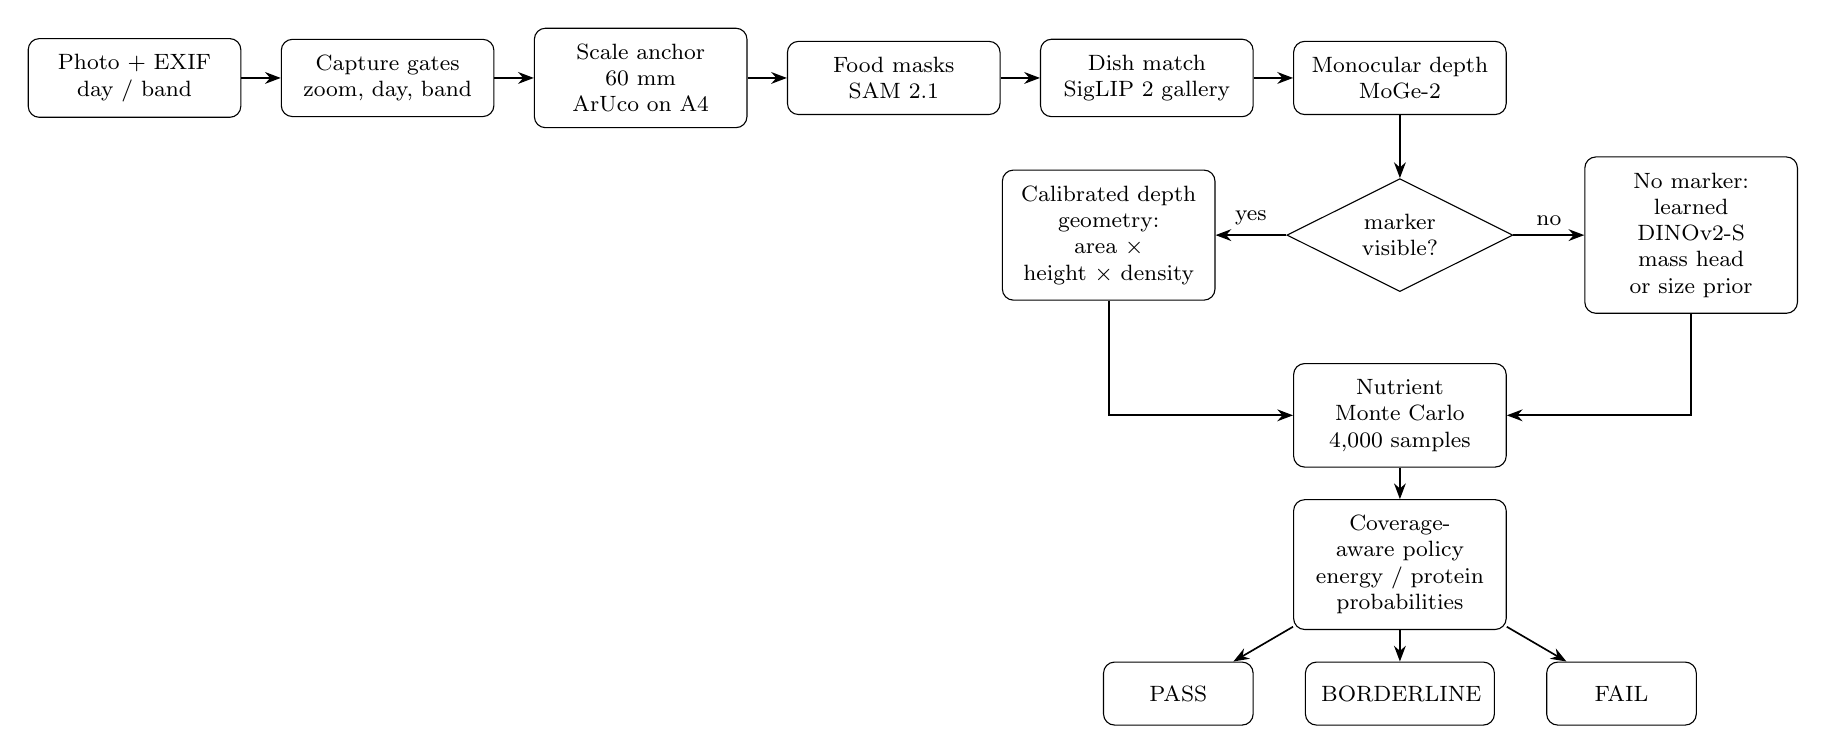
\begin{tikzpicture}[font=\footnotesize,node distance=4mm and 5mm,box/.style={draw,rounded corners,align=center,minimum height=8mm,text width=23mm,inner sep=2mm},decision/.style={draw,diamond,aspect=2,align=center,inner sep=1pt,text width=16mm},arrow/.style={-{Stealth[length=2mm]},semithick}]
\node[box](input){Photo + EXIF\\day / band};\node[box,right=of input](lint){Capture gates\\zoom, day, band};\node[box,right=of lint](anchor){Scale anchor\\60 mm ArUco on A4};\node[box,right=of anchor](seg){Food masks\\SAM 2.1};\node[box,right=of seg](cls){Dish match\\SigLIP 2 gallery};\node[box,right=of cls](depth){Monocular depth\\MoGe-2};
\draw[arrow](input)--(lint);\draw[arrow](lint)--(anchor);\draw[arrow](anchor)--(seg);\draw[arrow](seg)--(cls);\draw[arrow](cls)--(depth);
\node[decision,below=8mm of depth](tier){marker\\visible?};\draw[arrow](depth)--(tier);
\node[box,left=17mm and 9mm of tier](meas){Calibrated depth\\geometry: area $\times$\\height $\times$ density};\node[box,right=17mm and 9mm of tier](no){No marker: learned\\DINOv2-S mass head\\or size prior};\draw[arrow](tier)--node[above,sloped]{yes}(meas);\draw[arrow](tier)--node[above,sloped]{no}(no);
\node[box,below=9mm of tier](mc){Nutrient Monte Carlo\\4,000 samples};\draw[arrow](meas.south)|-(mc.west);\draw[arrow](no.south)|-(mc.east);
\node[box,below=of mc](policy){Coverage-aware policy\\energy / protein probabilities};\draw[arrow](mc)--(policy);
\node[box,below left=of policy,text width=15mm](out1){PASS};\node[box,below=of policy,text width=20mm](out2){BORDERLINE};\node[box,below right=of policy,text width=15mm](out3){FAIL};\draw[arrow](policy)--(out1);\draw[arrow](policy)--(out2);\draw[arrow](policy)--(out3);
\end{tikzpicture}}
\caption{NutriSense pipeline. Marker-calibrated geometry and no-marker mass estimation are distinct paths. Gate or stage failures abstain instead of producing a compliance score. No-marker results include an estimate disclaimer.}\label{fig:pipeline}\end{figure*}
\section{Methods}
\subsection{Scale, segmentation, and recognition}
The field reference is a 60\,mm ArUco ID 7 marker printed on A4 paper. Detection returns image-space corners and metric scale. The page format is A4; the marker side, not the sheet dimensions, anchors metric measurement. When detection fails, the system records a prior anchor rather than claiming measured scale.

SAM 2.1 generates dish masks. SigLIP 2 embeds each region for comparison with the 46-image gallery. The configured match threshold enables open-set abstention. The reported 46/46 gallery leave-one-out result is an internal gallery check, not independent test-set accuracy.
\subsection{Portion mass}
On the measured path, the system estimates volume from scale-adjusted footprint area and depth above an estimated plate or vessel base, then applies effective density $\rho_{\mathrm{eff}}$:
\begin{equation}m=V\rho_{\mathrm{eff}},\qquad V\approx A_{\mathrm{metric}}\bar{h}.\end{equation}
A ring near the mask boundary can estimate a base plane. Documented table or size priors are used when geometry is unavailable and are flagged as uncertain. Densities, dish shares, vessel parameters, and prior-tier values remain assumptions pending physical validation.

For mapped no-marker dishes, the model predicts mass directly from the crop and mask. It uses a frozen DINOv2-S/14 encoder, region feature pooling, and class-conditional regression trained on WED. It does not use monocular geometry to estimate grams. Per-class residual scale supplies mass uncertainty. If the head is unavailable or a dish is unmapped, the configured fallback and coverage penalty remain explicit.
\subsection{Nutrient uncertainty and compliance}
The system samples portion mass, recipe shares, configured nutrient values, and associated uncertainty using Monte Carlo ($n=4000$, fixed seed). For each mandatory nutrient it estimates probability $P$ that the meal reaches the applicable minimum. Coverage $C$ is a product of evidence-quality factors, including measured-anchor availability and whether mass came from a learned estimate or prior. PASS requires the configured probability and coverage minima; FAIL requires the corresponding low-probability and coverage criteria; BORDERLINE covers remaining scoreable cases. Invalid inputs, unsupported classes, and stage failures can abstain. No-marker responses lead with a disclaimer that mass is estimated. Salt is advisory and does not determine the verdict.
\section{Evaluation Protocol}
The repository evaluates image-region mass labels from WED, grouped by plate. Model selection uses a validation carve; the locked test split is protected. The current DINOv2-S result uses 108 validation views from 21 plates and 1,218 regions, seed 42, and 2,000 plate-bootstrap replicates. MAE is computed over regions:
\begin{equation}\mathrm{MAE}=\frac{1}{N}\sum_{i=1}^{N}|\hat m_i-m_i|.\end{equation}

Other results are separate component checks: SAM 2.1 IoU 0.98 on synthetic scenes; synthetic volume errors of +6.6\% (plate) and +5.6\% (bowl) with a card anchor; 1.1\% median marker-based MoGe depth-calibration error on rendered validation; and 46/46 gallery leave-one-out matches. These do not establish real-world end-to-end performance.
\section{Results}
The current DINOv2-S head achieved WED validation MAE 15.034\,g (plate-bootstrap 95\% CI [12.227, 18.889]\,g) over 1,218 regions on 21 plates. In paired evaluation on the same plates against the previous ResNet-50 head, MAE changed from 20.298 to 15.034\,g: $\Delta=-5.264$\,g (paired 95\% plate-bootstrap CI [$-6.232$, $-4.227$]). Estimated 90\% interval coverage was 0.8522 (95\% CI [0.792, 0.899]). This is development evidence and not a locked-test estimate.

The five recorded image perturbations also reduced validation MAE relative to the prior head in paired comparisons, though perspective perturbation remained harder (17.901\,g MAE). These perturbations are applied to validation images and are not naturally captured robustness data. Synthetic and gallery checks remain bounded to their own protocols.
\begin{table}[t]\caption{Current WED Validation Result}\label{tab:results}\centering\footnotesize\begin{tabular}{lc}\hline Measure&Result\\\hline Views / plates / regions&108 / 21 / 1,218\\DINOv2-S MAE&15.034 g\\Plate-bootstrap 95\% CI&[12.227, 18.889] g\\ResNet-50 baseline MAE&20.298 g\\Paired difference&$-5.264$ g\\Paired 95\% CI&[$-6.232$, $-4.227$] g\\90\% interval coverage&0.8522\\\hline\end{tabular}\end{table}
\section{Discussion and Limitations}
The evidence supports the feasibility of combining marker-based metric scale, visual mass regression, uncertainty propagation, and explicit policy gates in one software pipeline. The learned head improves validation MAE over the prior head on the same WED plates. This result is limited to a development carve and does not establish generalization to new institutions, dishes, cameras, serving conditions, or the protected test set.

Several stages remain weakly validated outside synthetic scenes. Gallery leave-one-out is small and not an independent classifier benchmark. Nutrient values, effective densities, recipe shares, vessel assumptions, no-marker calibration, coverage thresholds, and local PM POSHAN interpretation need review against measured meals and domain stakeholders. A single image can miss hidden food or confuse overlapping components. Accordingly, this work describes a software prototype, not a validated public-health measurement instrument.

Next steps are a controlled physical scale-and-weigh study, evaluation on locked data under the repository protocol, real-canteen measurements, nutrition-table validation, and coverage calibration. The A4 marker should be printed at its supplied page scale and physically checked.
\section{Conclusion}
NutriSense converts a meal photograph into dish-level mass estimates, nutrient intervals, and a coverage-aware assessment. It distinguishes measured scale from estimated no-marker mass. The DINOv2-S head achieved 15.034\,g WED validation MAE (95\% plate-bootstrap CI [12.227, 18.889]\,g), improving over its predecessor on paired validation plates. This does not establish test-set or field performance; physical and real-capture validation remain necessary.
\bibliographystyle{IEEEtran}\bibliography{references}
\end{document}
